\documentclass[../main.tex]{subfiles}

\graphicspath{{../images/}}

\begin{document}
\pagestyle{fancy}
\lhead{Homework 5}
\chead{Junseo Shin}
\rhead{PHYS 421}

\setcounter{section}{4}
% 3.16, 3.18, 3.25, 3.29, 3.38, 3.61

\paragraph{3.16} 

From Griffiths:
\begin{align*}
    V(x,y) = \frac{2V_0}{\pi} \arctan(\frac{\sin\pi y/a}{\sinh\pi x/a})
\end{align*}
where the surface charge density is given by a Gaussian pillbox
\begin{align*}
    \sigma = -\epsilon_0 \pdv{V}{n}
\end{align*}
since normal of the surface is $\vu{n} = \vu{x}$,
\begin{align*}
    \sigma &= -\epsilon_0 \pdv{x} \qt(
        \frac{2V_0}{\pi} \arctan(b)
    ) \\
    &= -\frac{2V_0 \epsilon_0}{\pi} \frac{1}{1 + b^2} \qt(\frac{-\sin(\pi y/a)}{\sinh^2(\pi x/a)}) \cosh(\pi x/a) \frac{\pi}{a} \\
    &= \frac{2V_0 \epsilon_0}{a} \frac{\sin(\pi y/a)}{\sinh^2(\pi x/a) + \sin^2(\pi y/a)} \cosh(\pi x/a)
\end{align*}
where at the boundary $x = 0$,
\begin{align*}
    \sinh(0) = 0, \cosh(0) = 1
\end{align*}
so 
\begin{align*}
    \sigma = \frac{2V_0 \epsilon_0}{a} \frac{\sin(\pi y/a)}{\sin^2(\pi y/a)} = \boxed{\frac{2V_0 \epsilon_0}{a} \sin(\pi y/a)}
\end{align*}

\newpage
\paragraph{3.18} Since only the top plate has a potential $V_0$ the boundary conditions are
\begin{enumerate}
    \item [(i)] $V = V_0$ at $z = a$
    \item [(ii)] $V = 0$ at $x = 0$, $y = 0$, $z = 0$, $x = a$, and $y = a$
\end{enumerate}
We look for solutions
\begin{align*}
    V(x,y,z) = X(x)Y(y)Z(z)
\end{align*}
and solving for Laplace's equation
\begin{align*}
    \frac{1}{X} \dv[2]{X}{x} + \frac{1}{Y} \dv[2]{Y}{y} + \frac{1}{Z} \dv[2]{Z}{z} = 0
\end{align*}
where
\begin{align*}
    \frac{1}{X} \dv[2]{X}{x} = C_1, \frac{1}{Y} \dv[2]{Y}{y} = C_2, \frac{1}{Z} \dv[2]{Z}{z} = C_3 \qqtext{with} C_1 + C_2 + C_3 = 0
\end{align*}
The textbook suggests that $C_1 = -k^2$, $C_2 = -l^2$, and $C_3 = k^2 + l^2$ where $k,l$ are constants. We can solve for $X,Y,Z$ separately:
\begin{align*}
    X(x) = A \sin(kx) + B \cos(kx) \\
    Y(y) = C \sin(ly) + D \cos(ly) \\
    Z(z) = E e^{\sqrt{k^2 + l^2} z} + F e^{-\sqrt{k^2 + l^2} z}
\end{align*}
So for the boundary conditions (ii) 
\begin{align*}
    \dv[2]{X}{x}\eval_{x = 0} &= - A^2 k^2 \sin^2(0) - B^2 k^2 \cos^2(0) = 0 \implies B = 0 \\
    \dv[2]{X}{x}\eval_{x = a} &= - A^2 k^2 \sin^2(ka) = 0 \implies k = \frac{n\pi}{a} \qq{for} n = 1,2,3,\cdots \\
    \dv[2]{Y}{y}\eval_{y = 0} &= - C^2 l^2 \sin^2(0) - D^2 l^2 \cos^2(0) = 0 \implies D = 0 \\
    \dv[2]{Y}{y}\eval_{y = a} &= - C^2 l^2 \sin^2(la) = 0 \implies l = \frac{m\pi}{a} \qq{for} m = 1,2,3,\cdots \\
    \dv[2]{Z}{z}\eval_{z = 0} &= E (k^2 + l^2) + F(k^2 + l^2)  = 0 \implies F = -E
\end{align*}
thus
\begin{align*}
    Z(z) &= E e^{\sqrt{k^2 + l^2} z} - E e^{-\sqrt{k^2 + l^2} z} \\
    &= 2E \sinh(\sqrt{k^2 + l^2} z) \\
    &= 2E \sinh(\sqrt{(\frac{n\pi}{a})^2 + (\frac{m\pi}{a})^2} z) \\
    &= 2E \sinh(\frac{\pi}{a} \sqrt{n^2 + m^2} z)
\end{align*}
The potential is now
\begin{align*}
    V(x,y,z) = \sum_{n=1}^\infty \sum_{m=1}^\infty C_{nm} \sin(\frac{n\pi x}{a}) \sin(\frac{m\pi y}{a}) \sinh(\frac{\pi}{a} \sqrt{n^2 + m^2} z)
\end{align*}
where we can solve for the Constants $C_{nm}$ using the boundary condition (i) $V = V_0$ at $z = a$:
\begin{align*}
    V_0 = \sum_{n=1}^\infty \sum_{m=1}^\infty C_{nm} \sin(\frac{n\pi x}{a}) \sin(\frac{m\pi y}{a}) \sinh(\frac{\pi}{a} \sqrt{n^2 + m^2} a)
\end{align*}
Doing the Fourier series by multiplying by $\sin(\frac{n'\pi x}{a}) \sin(\frac{m'\pi y}{a})$ and integrating over $x,y = [0,a]$:
\begin{align*}
    \int_0^a& \int_0^a V_0 \sin(\frac{n\pi x}{a}) \sin(\frac{m\pi y}{a}) \sin(\frac{n\pi x}{a}) \sin(\frac{m\pi y}{a}) dx dy \\
    &= \sum\sum C_{nm} \sinh(\frac{\pi}{a} \sqrt{n^2 + m^2} a) \int_0^a \int_0^a \sin^2(\frac{n\pi x}{a}) \sin^2(\frac{m\pi y}{a}) dx dy
\end{align*}
where the integral
\begin{align*}
    \int_0^a \sin(\frac{n\pi x}{a})\sin(\frac{n'\pi x}{a}) dx = \begin{cases}
        \frac{a}{2} & \text{if } n = n' \\
        0 & \text{if } n \neq n'
    \end{cases}
\end{align*}
So
\begin{align*}
    V_0 \int_0^a \int_0^a \sin(\frac{n\pi x}{a}) \sin(\frac{m\pi x}{a}) dx dy &= C_{nm} \sinh(\frac{\pi}{a} \sqrt{n^2 + m^2} a) \frac{a^2}{4}
\end{align*}
where
\begin{align*}
    C_{nm} \sinh(\frac{\pi}{a} \sqrt{n^2 + m^2} a) = \begin{cases}
        0 & \text{if } n \text{ or } m \text{ is even} \\
        \frac{16V_0}{\pi^2 n m} & \text{if } n \text{ and } m \text{ are odd}
    \end{cases}
\end{align*}
Thus the potential is
\begin{align*}
    \boxed{
        V(x,y,z) = \frac{16 V_0}{\pi^2} \sum_{n \text{ odd}} \sum_{m \text{ odd}} \frac{1}{nm} \sin(\frac{n\pi x}{a}) \sin(\frac{m\pi y}{a})
            \frac{\sinh(\frac{\pi}{a} \sqrt{n^2 + m^2} z)}{\sinh(\pi\sqrt{n^2 + m^2})}
    }
\end{align*}
The potential at the center is
\begin{align*}
    V(a/2, a/2, a/2) = \frac{16 V_0}{\pi^2} \sum_{n \text{ odd}} \sum_{m \text{ odd}} \frac{1}{nm} \sin(\frac{n\pi}{2}) \sin(\frac{m\pi}{2})
            \frac{\sinh(\frac{\pi}{a} \sqrt{n^2 + m^2} a/2)}{\sinh(\pi\sqrt{n^2 + m^2})}
\end{align*}
where a calculator gives us
\begin{align*}
    V(a/2, a/2, a/2) \approx 0.167 V_0
\end{align*}
Which roughly $V_0/6$ or a sixth of the potential in the center of a cube with $V_0$ on each face.

\newpage
\paragraph{3.25} The potential inside and outside the sphere is given by (Griffiths 3.78 \& 3.79)
\begin{align*}
    V(r,\theta) = \begin{cases}
        \sum_{l=0}^\infty A_l r^l P_l(\cos\theta) & (r \leq R) \\
        \sum_{l=0}^\infty \frac{B_l}{r^{l+1}} P_l(\cos\theta) & (r \geq R)
    \end{cases}
\end{align*}
where (3.81 \& 3.84)
\begin{align*} \tag{3.81}
    B_l = A_l R^{2l + 1}
\end{align*}
\begin{align*} \tag{3.84}
    A_l = \frac{1}{2\epsilon_0 R^{l-1}} \int_0^\pi  \sigma_0(\theta) P_l (\cos\theta) \sin\theta d\theta
\end{align*}
Since the charge density is constant $\sigma_0(\theta) = \sigma_0$ and using $u = \cos\theta; \cos(0) = 1, \cos(\pi) = -1$ and $du = -\sin\theta d\theta$ we get
\begin{align*}
    A_l &= -\frac{\sigma_0}{2\epsilon_0 R^{l-1}} \int_1^{-1} P_l(u) du
\end{align*}
where $P_l(u)$ is odd for odd $l$ and even for even $l$ so the integral is zero for odd $l$ and non-zero for even $l$:
\begin{align*}
    \int_1^{-1} P_l(u) du = \begin{cases}
        0 & \text{if } l \text{ is even} \\
        -2 \int_0^1 P_l(u) du & \text{if } l \text{ is odd}
    \end{cases}
\end{align*}
Thus
\begin{align*}
    A_l = -\frac{\sigma_0}{2\epsilon_0 R^{l-1}} (-2)\int_0^1 P_l(u) du = \begin{cases}
        0 & \text{if } l \text{ is odd} \\
        \frac{\sigma_0}{\epsilon_0 R^{l-1}} \int_0^1 P_l(u) du & \text{if } l \text{ is even}
    \end{cases}
\end{align*}
So for the odd $P_l$
\begin{align*}
    \int_0^1 P_1(u) du &= \int_0^1 u du = \frac{1}{2} \\
    \int_0^1 P_3(u) du &= \frac{1}{2} \int_0^1 (5u^3 - 3u) du = -\frac{1}{8} \\
    \int_0^1 P_5(u) du &= \frac{1}{8} \int_0^1 (63u^5 - 70u^3 + 15u) du = \frac{1}{16}
\end{align*}
and for the even $P_l$ the integral is zero; therfore
\begin{gather*}
    A_0 = A_2 = A_4 = A_6 = 0 \\
    A_1 = \frac{\sigma_0}{\epsilon_0} \frac{1}{2}, \quad A_3 = \frac{\sigma_0}{\epsilon_0 R^2} \qt(\frac{-1}{8}), \quad A_5 = \frac{\sigma_0}{\epsilon_0 R^4} \frac{1}{16}
\end{gather*}
and 
\begin{gather*}
    B_0 = B_2 = B_4 = B_6 = 0 \\
    B_1 = \frac{\sigma_0}{\epsilon_0} R^3 \frac{1}{2}, \quad B_3 = \frac{\sigma_0}{\epsilon_0} R^5 \qt(\frac{-1}{8}), \quad B_5 = \frac{\sigma_0}{\epsilon_0} R^7 \frac{1}{16}
\end{gather*}
So finally the potential is
\begin{align*}
    \boxed{
        V(r, \theta) = \frac{\sigma_0}{\epsilon_0} \qt[
            \frac{r}{2} P_1(\cos\theta) - \frac{r^3}{8R^2} P_3(\cos\theta) + \frac{r^5}{16R^4} P_5(\cos\theta)
        ] \quad (r \leq R)
    }
\end{align*}
and 
\begin{align*}
    \boxed{
        V(r, \theta) = \frac{\sigma_0}{\epsilon_0} \qt[
            \frac{R^3}{2r^2} P_1(\cos\theta) - \frac{R^5}{8r^4} P_3(\cos\theta) + \frac{R^7}{16r^6} P_5(\cos\theta)
        ] \quad (r \geq R)
    }
\end{align*}

\newpage
\paragraph{3.29} Given charge density
\begin{align*}
    \rho(r, \theta) = k \frac{R}{r^2} (R - 2r) \sin\theta
\end{align*}
for a sphere of radius $R$ and constant $k$. The monopole term is
\begin{align*}
    \int \rho \dd\tau = kR \int \qt(
        \frac{1}{r^2}{R - 2r} \sin\theta
    ) r^2 \sin\theta dr d\theta d\phi
\end{align*}
Where the radial integral is
\begin{align*}
    \int_0^R R - 2r dr = 0
\end{align*}
Moving on to the dipole term
\begin{align*}
    \int r \cos\theta \rho \dd\tau = kR \int (r\cos\theta) (R - 2r) \sin\theta \sin\theta dr d\theta d\phi
\end{align*}
where the polar integral is
\begin{align*}
    \int_0^\pi \sin\theta \cos\theta d\theta = 0
\end{align*}
Maybe the quadrupole term will be non-zero:
\begin{align*}
    \int r^2 \qt(
        \frac{3}{2} \cos^2\theta - \frac{1}{2}) \rho \dd\tau &= \frac{1}{2} kR \int_0^{2\pi} \int_0^\pi \int_0^R r^2 \qt(
                (3\cos^2\theta - 1) (R - 2r) \sin\theta) dr d\theta d\phi \\
    &= \frac{1}{2} kR (2\pi) \qt(-\frac{\pi}{8}) \qt(-\frac{R^4}{6}) \\
    &= \frac{\pi^2 k R^5}{48}
\end{align*}
So far from the sphere for points on the $z$-axis the potential is
\begin{align*}
    \boxed{
        V(z) = \ke \frac{\pi^2 K R^5}{48 z^3}
    }
\end{align*}

\newpage 
\paragraph{3.38} Given
\begin{align*}\tag{3.103} \label{eq:3.103}
    \vb E_\text{dip} (r,\theta) = \frac{p}{4\pi\epsilon_0 r^3} (2\cos\theta \vu{r} + \sin\theta \vu{\theta})
\end{align*}
and
\begin{align*}\tag{3.104} \label{eq:3.104}
    \vb E_\text{dip} (r,\theta) = \ke \frac{1}{r^3} [3(\vb p \cdot \vu r) \vu r - \vb p]
\end{align*}
The dipole moment has vector components
\begin{align*}
    \vb p = p \cos\theta \vu r + p \sin\theta \vu\theta
\end{align*}
so now we can sub this into \eqref{eq:3.104}:
\begin{align*}
    \vb E_\text{dip} (r,\theta) &= \ke \frac{1}{r^3} [3(\vb p \cdot \vu r) \vu r - \vb p] \\
    &= \ke \frac{1}{r^3} 3(p \cos\theta) \vu r - (p \cos\theta \vu r + p \sin\theta \vu\theta) \\
    \textrm{Eq. 3.103} &= \frac{p}{4\pi \epsilon_0 r^3} (2 \cos\theta \vu r - \sin\theta \vu\theta)
\end{align*}

\newpage
\begin{figure*}[ht]
    \centering
    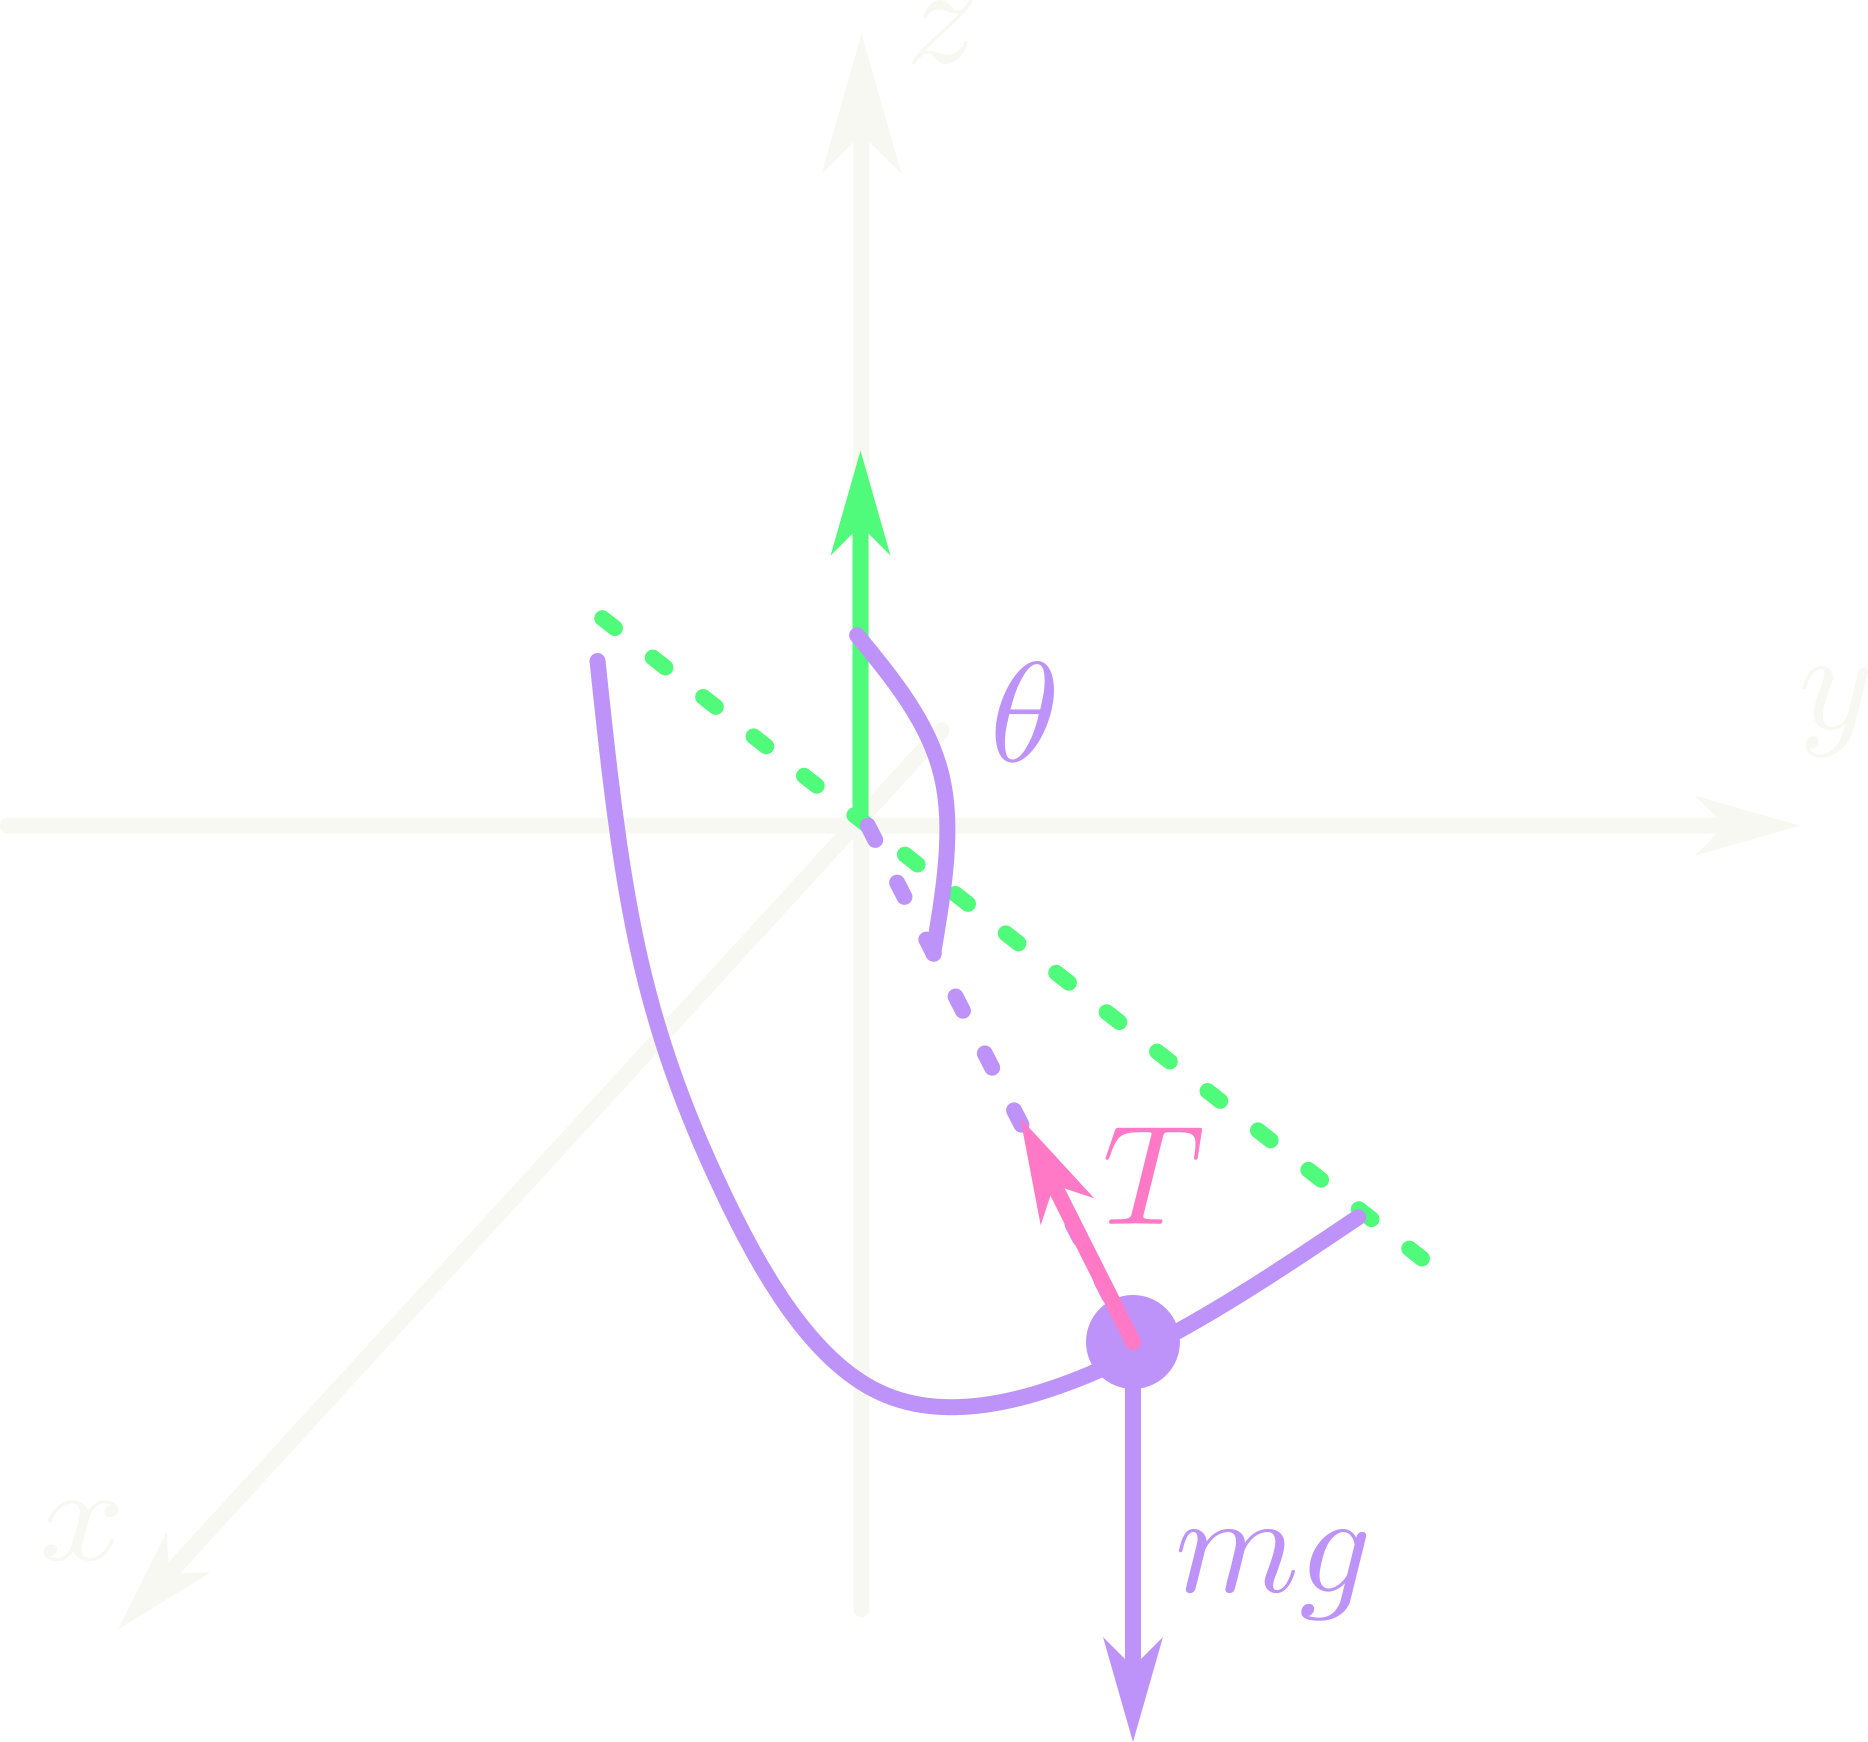
\includegraphics[width=0.5\linewidth]{hw4.png}
    \caption{The electric field of a dipole at a distance $r$ from the origin.}
    \label{fig:hw5_3_38}
\end{figure*}
\paragraph{3.61} Given the potential from \eqref{eq:3.103} and the force
\begin{align*}
    \vb F = q\vb E = \frac{qp}{4\pi\epsilon_0 r^3} (2\cos\theta \vu r + \sin\theta \vu\theta)
\end{align*}
Pretending this is a pendulum as shown in Fig. \ref{fig:hw5_3_38} the force is
\begin{align*}
    \vb F = - T \vu r - mg \vu z = - T \vu r - mg (\cos\theta \vu r - \sin\theta \vu\theta)
\end{align*}
$T$ is the tension given by the centripetal acceleration
\begin{gather*}
    m a_c = T - mg \cos(\pi - \theta) \\
    m\frac{v^2}{r} = T + mg \cos\theta
\end{gather*}
where $v$ is the velocity given by energy conservation
\begin{align*} 
    KE &= \Delta PE \\
    \frac{1}{2} m v^2 &= -mg r \cos\theta \\
    \implies v^2 &= -2g r \cos\theta
\end{align*}
So
\begin{align*}
    T = m\frac{v^2}{r} - mg \cos\theta = -2mg \cos\theta - mg \cos\theta  = -3mg \cos\theta
\end{align*}
Thus we get the force 
\begin{align*}
    \vb F &= 3mg \cos\theta \vu r - mg(\cos\theta \vu r - \sin\theta \vu\theta) \\
    &= mg (2\cos\theta \vu r + \sin\theta \vu\theta)
\end{align*}
Which is telling us that the electric charge will swing in an arc like a pendulum i.e.
\begin{align*}
    mg \equiv \frac{qp}{4\pi\epsilon_0 r^3}
\end{align*}
or we can think of the charge $q$ as an inertial mass and group the other terms as the gravitational constant.

\end{document}